% Created 2016-06-20 一 08:35
\documentclass[xcolor=svgnames,presentation]{beamer}
\usepackage[utf8]{inputenc}
\usepackage[T1]{fontenc}
\usepackage{fixltx2e}
\usepackage{graphicx}
\usepackage{longtable}
\usepackage{float}
\usepackage{wrapfig}
\usepackage{soul}
\usepackage{textcomp}
\usepackage{marvosym}
\usepackage{wasysym}
\usepackage{latexsym}
\usepackage{amssymb}
\usepackage{hyperref}
\tolerance=1000
\usepackage{minted}
\usecolortheme[named=FireBrick]{structure}\setbeamercovered{transparent}\setbeamertemplate{caption}[numbered]\setbeamertemplate{blocks}[rounded][shadow=true] \usetheme{Darmstadt}\date{\today} \usepackage{tikz}\usepackage{xeCJK}\usepackage{amsmath}\setmainfont{Times New Roman}\setCJKmainfont[BoldFont={Adobe Heiti Std},ItalicFont={Adobe Fangsong Std}]{Adobe Heiti Std}\setCJKsansfont{Adobe Heiti Std}\setCJKmonofont{Adobe Fangsong Std}\usepackage{verbatim}\graphicspath{{figures/}} \definecolor{lstbgcolor}{rgb}{0.9,0.9,0.9} \usepackage{listings}\usepackage{minted} \usepackage{fancyvrb}\usepackage{xcolor}\lstset{escapeinside=`',frameround=ftft,language=C,breaklines=true,keywordstyle=\color{blue!70},commentstyle=\color{red!50!green!50!blue!50},frame=shadowbox,backgroundcolor=\color{yellow!20},rulesepcolor=\color{red!20!green!20!blue!20}}
\usemintedstyle{default}
\providecommand{\alert}[1]{\textbf{#1}}

\title{第2讲 Linux基础}
\author{王晓庆}
\date{\today}
\hypersetup{
  pdfkeywords={},
  pdfsubject={},
  pdfcreator={Emacs Org-mode version 7.9.3f}}

\institute{wangxiaoqing@outlook.com}
\begin{document}

\maketitle

\begin{frame}
\frametitle{Outline}
\setcounter{tocdepth}{1}
\tableofcontents
\end{frame}

\section{Linux文件管理}
\label{sec-1}
\subsection{文件和目录管理}
\label{sec-1-1}
\begin{frame}[fragile]
\frametitle{创建文件和目录}
\label{sec-1-1-1}
\begin{exampleblock}{创建文件}
\label{sec-1-1-1-1}


\begin{minted}[]{bash}
ed f1           #用编辑器创建f1
a    #添加append
Ed is a line-oriented text editor of Unix.
It is old, simple and fun.
.    #结束输入
w    #存盘
q    #退出
touch f{1..9}   #更新f1,创建空文件f2,...,f9
\end{minted}
\end{exampleblock}
\begin{block}{创建目录}
\label{sec-1-1-1-2}


\begin{minted}[]{bash}
mkdir d{1..9}               #创建多个目录
mkdir -p dir1/dir2/dir3     #按路径创建多层目录
\end{minted}
\end{block}
\end{frame}
\begin{frame}[fragile]
\frametitle{复制文件和目录}
\label{sec-1-1-2}
\begin{exampleblock}{复制文件}
\label{sec-1-1-2-1}


\begin{minted}[]{bash}
cp f1 f1.1                 #把f1复制为f1.1
cp -i f1 f2                #覆盖时提示
cp -p f1 f1.2              #保留文件属性不变
cp f3 f4 dir1              #把文件复制到目录
cp -p f3 dir1/dir22/f3.1   #把文件复制到目录并改名
\end{minted}
\end{exampleblock}
\begin{block}{复制目录}
\label{sec-1-1-2-2}


\begin{minted}[]{bash}
cp x/* da                  #复制目录内所有文件
cp -R x db                 #递归复制整个目录
cp -a x dc                 #同上并保留文件属性不变
\end{minted}
\end{block}
\end{frame}
\begin{frame}[fragile]
\frametitle{移动文件和目录}
\label{sec-1-1-3}
\begin{exampleblock}{移动文件}
\label{sec-1-1-3-1}


\begin{minted}[]{bash}
mv f4 f4.1           #将f4移动(重命名)为f4.1
mv f5 d3             #将文件移动到目录
mv -i f5 f6          #覆盖时提示
mv f6 c/f6.1         #移动并改名
mv  *.1 d4           #将文件移动到目录
\end{minted}
\end{exampleblock}
\begin{block}{移动目录}
\label{sec-1-1-3-2}


\begin{minted}[]{bash}
mv d4 dir1/dir2      #目录移动
mv d5 d05            #目录改名
\end{minted}
\end{block}
\end{frame}
\begin{frame}[fragile]
\frametitle{删除文件和目录}
\label{sec-1-1-4}
\begin{exampleblock}{删除文件}
\label{sec-1-1-4-1}


\begin{minted}[]{bash}
rm f8 f9                  #删除文件f8、f9
rm -i f7                  #删除前确认
rm -f f*                  #强行删除
\end{minted}
\end{exampleblock}
\begin{block}{删除目录}
\label{sec-1-1-4-2}


\begin{minted}[]{bash}
rmdir d7 d8               #删除空目录
rmdir -p dir1/dir2/dir3   #删除多层空目录
rm -r d6 dir1             #删除目录
rm -rf /                  #删除所有文件!!!
\end{minted}
\end{block}
\end{frame}
\begin{frame}[fragile]
\frametitle{判断文件类型}
\label{sec-1-1-5}
\begin{exampleblock}{file}
\label{sec-1-1-5-1}


\begin{minted}[]{bash}
file /etc/hosts
file /usr/bin/cat
file /var
file /dev/sda1
\end{minted}
\end{exampleblock}
\end{frame}
\begin{frame}[fragile]
\frametitle{文件查找}
\label{sec-1-1-6}
\begin{itemize}

\item which
\label{sec-1-1-6-1}%
\begin{itemize}

\item 在\$PATH列出的目录中查找可执行程序,并返回第一个匹配结果或返回未找到提示\\
\label{sec-1-1-6-1-1}%
\begin{minted}[]{bash}
which mkdir
\end{minted}
\end{itemize} % ends low level

\item whereis
\label{sec-1-1-6-2}%
\begin{itemize}

\item 在某些特定目录中查找可执行程序、源码及软件文档\\
\label{sec-1-1-6-2-1}%
\begin{minted}[]{bash}
whereis -l       #列出whereis的搜索目录列表
whereis mkdir
\end{minted}
\end{itemize} % ends low level

\item locate
\label{sec-1-1-6-3}%
\begin{itemize}

\item 在系统定期更新的索引数据库中检索文件
\label{sec-1-1-6-3-1}%

\item 查找速度快,但索引数据库不会实时更新
\label{sec-1-1-6-3-2}%

\item 可通过执行updatedb手动更新索引数据库\\
\label{sec-1-1-6-3-3}%
\begin{minted}[]{bash}
locate hosts
touch newfile
locate newfile
\end{minted}
\end{itemize} % ends low level
\end{itemize} % ends low level
\end{frame}
\begin{frame}[fragile]
\frametitle{文件查找}
\label{sec-1-1-7}
\begin{itemize}

\item find
\label{sec-1-1-7-1}%
\begin{itemize}

\item 功能强大,可根据各种复杂条件进行文件查找
\label{sec-1-1-7-1-1}%

\item 对目录进行递归遍历,速度慢,应该尽量缩小查找范围
\label{sec-1-1-7-1-2}%
\end{itemize} % ends low level
%% 示例
\label{sec-1-1-7-1-3}


\begin{minted}[]{bash}
find /usr/bin -name chmod -print #找文件chmod
find /usr/bin -name "ch*"        #找ch开头的文件
find /usr/bin -size 5M           #找5MB大小的文件
find /usr/bin -size +5M          #找大于5MB的文件
find /usr/bin -size -5M          #找小于5MB的文件
find /usr/bin ! -size -5M       #找不小于5MB文件
find /usr/bin -size +5M -exec ls -sh {} \; 
#对找到的文件执行相应操作
find /usr/bin -size +5M -a -size -9M -exec ls -sh {} \; 
#多条件联合查找,-a(-and)可省略,还支持-o(-or)、!(-not)
\end{minted}
\end{itemize} % ends low level
\end{frame}
\begin{frame}[fragile]
\frametitle{文件查找}
\label{sec-1-1-8}
%% find
\label{sec-1-1-8-1}


\begin{minted}[]{bash}
find . -type -f -mtime +1 -exec ls -lt {} \; 
#查找过去48小时之前修改过的文件
find . -type -f -mtime 1 -exec ls -lt {} \;  
#查找过去24小时之前,48小时之内修改过的文件
find . -type -f -mtime -1 -exec ls -lt {} \; 
#查找过去24小时之内修改过的文件
find . -type -f -mtime +0 -exec ls -lt {} \; 
#查找过去24小时之前修改过的文件
find . -type -f -mtime 0 -exec ls -l {} \;   
#查找现在之前,过去24小时内修改过的文件
find . -type -f -mtime -0 -exec ls -l {} \;  
#查找现在之后修改过的文件
find . -type -f -mtime +0 -mtime -2 -ok cp -l {}  ~/bak \; 
#查找过去24小时之前,48小时之内修改过的文件
\end{minted}
\note{备注


\begin{minted}[]{bash}
find . -type f -mtime +2 -exec ls -lt {} \;  #过去72小时之前
find . -type f -mtime 2 -exec ls -lt {} \;   #过去48小时之前,72小时之内
find . -type -f -mtime -2 -exec ls -lt {} \; #过去48小时之内

find . -type -f -mtime +1 -exec ls -lt {} \; #过去48小时之前
find . -type -f -mtime 1 -exec ls -lt {} \;  #过去24小时之前,48小时之内
find . -type -f -mtime -1 -exec ls -lt {} \; #过去24小时之内

find . -type -f -mtime +0 -exec ls -lt {} \; #过去24小时之前
find . -type -f -mtime 0 -exec ls -l {} \;   #现在之前,过去24小时内
find . -type -f -mtime -0 -exec ls -l {} \;  #现在之后

find . -type -f -mtime +0 -mtime -2 -ok cp -l {}  ~/bak \; #过去24小时之前,48小时之内
\end{minted}
}
\end{frame}
\begin{frame}
\frametitle{查找文件}
\label{sec-1-1-9}
\begin{itemize}

\item 查找时间示意图(图中每一小段代表24小时)\\
\label{sec-1-1-9-1}%
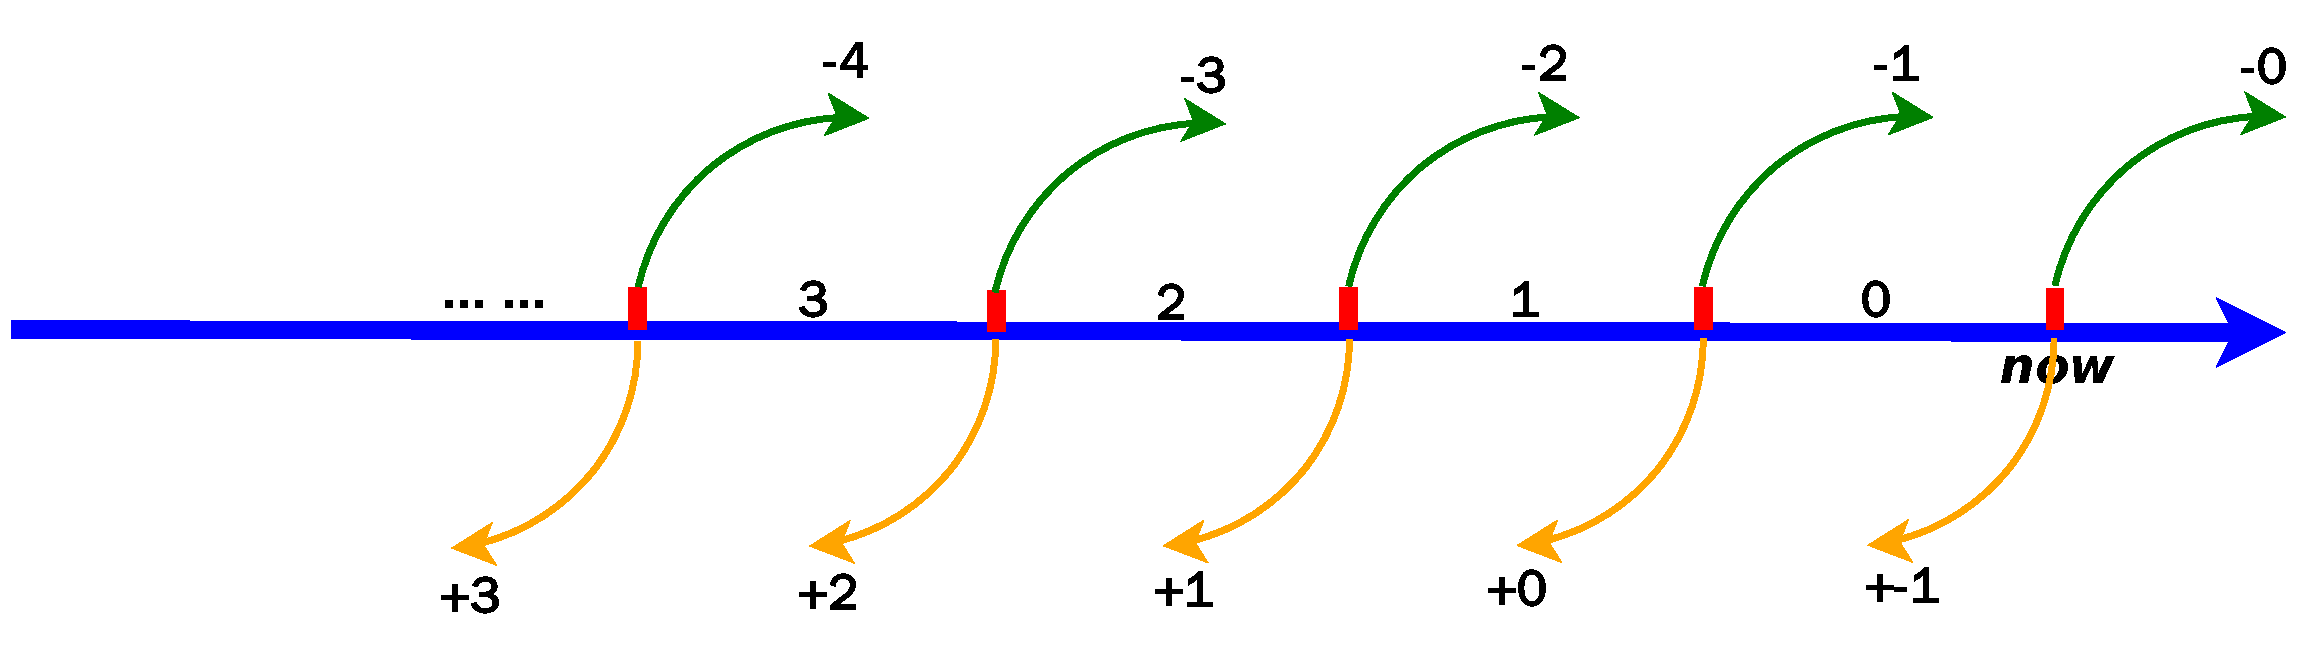
\includegraphics[width=.9\linewidth]{img/find-time.pdf}
\end{itemize} % ends low level
\end{frame}
\begin{frame}[fragile]
\frametitle{文件内容计数}
\label{sec-1-1-10}
\begin{itemize}

\item wc
\label{sec-1-1-10-1}%
\end{itemize} % ends low level
\begin{exampleblock}{示例}
\label{sec-1-1-10-2}


\begin{minted}[]{bash}
wc learn-vim
wc -l learn-vim
wc -w learn-vim
wc -c learn-vim
\end{minted}
\end{exampleblock}
\end{frame}
\begin{frame}[fragile]
\frametitle{文件内容搜索}
\label{sec-1-1-11}
\begin{itemize}

\item grep
\label{sec-1-1-11-1}%
\end{itemize} % ends low level
\begin{exampleblock}{示例}
\label{sec-1-1-11-2}


\begin{minted}[]{bash}
grep root /etc/passwd
grep "insert mode" learn-vim
grep -i "insert mode" learn-vim
grep -n "insert mode" learn-vim
grep -vn "nologin" /etc/passwd
grep -c "/bin/bash" /etc/passwd
\end{minted}
\end{exampleblock}
\end{frame}
\section{shell及其特性}
\label{sec-2}
\subsection{shell}
\label{sec-2-1}
\begin{frame}[fragile]
\frametitle{查看和设置登录shell}
\label{sec-2-1-1}


\begin{minted}[]{bash}
echo $SHELL              #打印当前shell路径
chsh -l                  #列出系统可用shell列表
chsh -s /bin/csh         #指定登录shell,下次登录生效
\end{minted}
\end{frame}
\begin{frame}[fragile]
\frametitle{文件名通配符}
\label{sec-2-1-2}
\begin{exampleblock}{* 代表0到多个任意字符(换行符除外)}
\label{sec-2-1-2-1}


\begin{minted}[]{bash}
ls file*
\end{minted}
\end{exampleblock}
\begin{block}{? 代表1个任意字符(换行符除外)}
\label{sec-2-1-2-2}


\begin{minted}[]{bash}
ls file?
\end{minted}
\end{block}
\begin{exampleblock}{[xyz] 代表1个指定范围内字符}
\label{sec-2-1-2-3}


\begin{minted}[]{bash}
ls file[123]
ls file[0-9][ab]
ls file[^0-9]
ls file[!23]
\end{minted}
\end{exampleblock}
\begin{itemize}

\item 注意:文件名通配符只能匹配已经存在的文件名!
\label{sec-2-1-2-4}%
\end{itemize} % ends low level
\end{frame}
\begin{frame}
\frametitle{标准I/O文件}
\label{sec-2-1-3}
\begin{itemize}

\item shell会为每个进程打开三个文件
\label{sec-2-1-3-1}%
\begin{enumerate}
\item 标准输入(stdin):文件描述符为0,默认指向键盘
\item 标准输出(stdout):文件描述符为1,默认指向显示屏
\item 标准错误(stderr):文件描述符为2,默认指向显示屏
\end{enumerate}
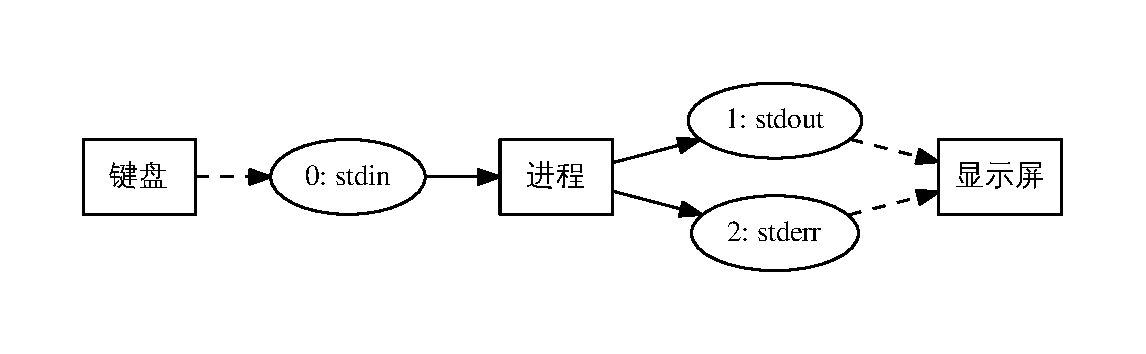
\includegraphics[width=.9\linewidth]{img/stdio.pdf}
\end{itemize} % ends low level
\end{frame}
\begin{frame}[fragile]
\frametitle{标准输入重定向}
\label{sec-2-1-4}
\begin{exampleblock}{示例}
\label{sec-2-1-4-1}


\begin{minted}[]{bash}
cat
cat <students.db
mail alice bob tom mary <letter
\end{minted}
\end{exampleblock}
\begin{block}{想一想}
\label{sec-2-1-4-2}


\begin{verbatim}
以下两条命令有何区别?
wc file
wc <file
\end{verbatim}
\end{block}
\end{frame}
\begin{frame}[fragile]
\frametitle{标准输出重定向}
\label{sec-2-1-5}
\begin{exampleblock}{示例}
\label{sec-2-1-5-1}


\begin{minted}[]{bash}
ls
ls >ls.out
cat file1 file2
cat file1 file2 >allfiles
cat file3 >>allfiles
who >temp
wc -l <temp
cat <file1 >file2
\end{minted}
\end{exampleblock}
\begin{block}{想一想}
\label{sec-2-1-5-2}


\begin{verbatim}
1. 为什么ls >ls.out会导致ls.out包括在名单中?
2. 执行wc temp >temp后,temp文件的内容是什么?
3. 如果拼错了命令名,比如woh >temp,会发生什么?
\end{verbatim}
\end{block}
\end{frame}
\begin{frame}[fragile]
\frametitle{标准错误重定向}
\label{sec-2-1-6}
\begin{exampleblock}{示例}
\label{sec-2-1-6-1}


\begin{minted}[]{bash}
ls .bashrc .profile >ls.out
ls .bashrc .profile 2>ls.err
ls .bashrc .profile 2>/dev/null #抛弃错误输出
ls memo.1 memo.2 2>>ls.err
ls .bashrc .profile >ls.out 2>ls.err
ls .bashrc .profile >ls.out 2>&1
ls .bashrc .profile 2>&1 >ls.out
ls .bashrc .profile &>ls.out #也可写成>&
ls .bash_profile memo.1 &>>ls.out
\end{minted}
\end{exampleblock}
\end{frame}
\begin{frame}[fragile]
\frametitle{管道}
\label{sec-2-1-7}
\begin{itemize}

\item 通过管道可以将一个程序的标准输出连接到另一个程序的标准输入\\
\label{sec-2-1-7-1}%
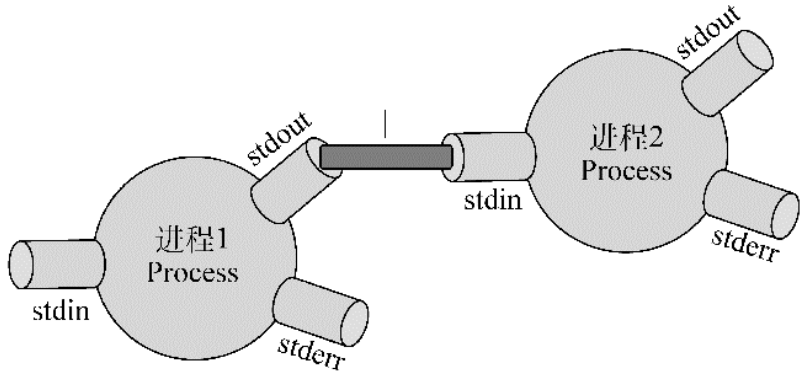
\includegraphics[width=.9\linewidth]{img/pipe.png}
\end{itemize} % ends low level
\begin{exampleblock}{示例}
\label{sec-2-1-7-2}


\begin{minted}[]{bash}
who | sort
\end{minted}
\end{exampleblock}
\end{frame}
\begin{frame}[fragile]
\frametitle{管道}
\label{sec-2-1-8}
\begin{exampleblock}{示例}
\label{sec-2-1-8-1}


\begin{minted}[]{bash}
who | wc -l
ls | wc -l
who | grep xiaobai | wc -l
\end{minted}
\end{exampleblock}
\begin{block}{想一想}
\label{sec-2-1-8-2}


\begin{verbatim}
下面两条命令有何不同?
who | sort
who >sort
\end{verbatim}
\end{block}
\begin{exampleblock}{tee:T形管道}
\label{sec-2-1-8-3}


\begin{minted}[]{bash}
who | tee who.out | grep xiaobai | tee grep.out | wc -l
\end{minted}
\end{exampleblock}
\end{frame}
\section{文本处理工具}
\label{sec-3}
\subsection{常用文本处理命令}
\label{sec-3-1}
\begin{frame}[fragile]
\frametitle{cut:列截取}
\label{sec-3-1-1}
\begin{exampleblock}{示例文件:students.db}
\label{sec-3-1-1-1}


\begin{verbatim}
1 mary female 19 100
2 tom male 20 93
3 susie female 20 97
4 bob male 21 90
5 alice female 18 92
6 mike male 19 89
\end{verbatim}
\end{exampleblock}
\begin{block}{示例}
\label{sec-3-1-1-2}


\begin{minted}[]{bash}
cut -c3 students.db
cut -c3-7 students.db
cut -d' ' -f2,5 students.db
\end{minted}
\end{block}
\note{students.db


\begin{verbatim}
students.db
1 mary female 19 100
2 tom male 20 93
3 susie female 20 97
4 bob male 21 90
5 alice female 18 92
6 mike male 19 89
students2.db
1,mary,female,19,100
2,tom,male,20,93
3,susie,female,20,97
4,bob,male,21,90
5,alice,female,18,92
6,mike,male,19,89
\end{verbatim}
}
\end{frame}
\begin{frame}[fragile]
\frametitle{sort:排序}
\label{sec-3-1-2}
\begin{exampleblock}{示例文件:students2.db}
\label{sec-3-1-2-1}


\begin{verbatim}
All the light we cannot see^Anthony Doerr^2014^$15.29
Red queen^Victoria Aveyard^2015^$10.58
Saga,Vol.1^Brian K. Vaughan^2012^$8.46
The blood of Olympus^Pick Piordan^2014^$11.99
The day the crayons quit^Drew Daywalt^2013^$10.32
The girl on the train^Paula Hawkins^2015^$14.01
Winter(Lunar)^Marissa Meyer^2015^$13.84
\end{verbatim}
\end{exampleblock}
\begin{block}{示例}
\label{sec-3-1-2-2}


\begin{minted}[]{bash}
sort books.db                #按字典序排序
sort -t^ -k3 books.db        #按出版年份排序
sort -t^ -k4.2 books.db      #根据价格排序:-(
sort -t^ -k4.2 -nr books.db  #根据价格逆序排序:-)
\end{minted}
\end{block}
\note{备忘


\begin{minted}[]{bash}
sort -m file1 file2 >file12  #合并排序后的文件
sort -u file1 >file1.u       #排序后删除重复行
\end{minted}
}
\end{frame}
\begin{frame}[fragile]
\frametitle{uniq:消除相邻重复行}
\label{sec-3-1-3}
\begin{exampleblock}{示例文件:numbers}
\label{sec-3-1-3-1}


\begin{verbatim}
123
56
123
123
78
78
30
\end{verbatim}
\end{exampleblock}
\begin{block}{示例}
\label{sec-3-1-3-2}


\begin{minted}[]{bash}
uniq numbers
sort numbers | uniq
uniq -c numbers.sort
\end{minted}
\end{block}
\end{frame}
\begin{frame}[fragile]
\frametitle{join:行连接}
\label{sec-3-1-4}
%% 示例文件
\label{sec-3-1-4-1}
\begin{columns}
\begin{column}{0.5\textwidth}
\begin{exampleblock}{file1}
\label{sec-3-1-4-1-1}


\begin{verbatim}
1 tom
2 mary
3 bob
4 susie
5 alice
6 mike
\end{verbatim}
\end{exampleblock}
\end{column}
\begin{column}{0.5\textwidth}
\begin{exampleblock}{file2}
\label{sec-3-1-4-1-2}


\begin{verbatim}
tom 98
mary 100
alice 96
mike 90
susie 93
bob 88
\end{verbatim}
\end{exampleblock}
\end{column}
\end{columns}
\begin{block}{示例}
\label{sec-3-1-4-2}


\begin{minted}[]{bash}
sort -k 2 file1 >file1.s
sort file2 >file2.s
join -12 -21 file1.s file2.s
\end{minted}
\end{block}
\end{frame}
\begin{frame}[fragile]
\frametitle{paste:列合并}
\label{sec-3-1-5}
%% 示例文件
\label{sec-3-1-5-1}
\begin{columns}
\begin{column}{0.5\textwidth}
\begin{exampleblock}{file1}
\label{sec-3-1-5-1-1}


\begin{verbatim}
1 tom
2 mary
3 bob
4 susie
5 alice
6 mike
\end{verbatim}
\end{exampleblock}
\end{column}
\begin{column}{0.5\textwidth}
\begin{exampleblock}{file3}
\label{sec-3-1-5-1-2}


\begin{verbatim}
male 23
female 22
male 21
female 20
female 19
male 20
\end{verbatim}
\end{exampleblock}
\end{column}
\end{columns}
%% 示例
\label{sec-3-1-5-2}
\begin{block}{示例}
\label{sec-3-1-5-2-1}


\begin{minted}[]{bash}
paste file1 file3
paste -d' ' file1 file3
\end{minted}
\end{block}
\end{frame}
\begin{frame}[fragile]
\frametitle{压缩和解压}
\label{sec-3-1-6}
\begin{exampleblock}{gzip}
\label{sec-3-1-6-1}


\begin{minted}[]{bash}
gzip file1 file2             #压缩
gzip -d file1.gz file2.gz    #解压缩
gunzip file1.gz file2.gz     #解压缩
\end{minted}
\end{exampleblock}
\begin{block}{bzip2}
\label{sec-3-1-6-2}


\begin{minted}[]{bash}
bzip2 file1 file2            #压缩
bzip2 -d file1.bz2 file2.bz2 #解压缩
bunzip2 file1.bz2 file2.bz2  #解压缩
\end{minted}
\end{block}
\begin{exampleblock}{zip}
\label{sec-3-1-6-3}


\begin{minted}[]{bash}
zip zipfile1 file1 file2     #压缩文件(不要加.zip后缀)
zip -r zipdir1 dir1          #压缩目录
unzip zipdir1.zip            #解压缩
\end{minted}
\end{exampleblock}
\end{frame}
\begin{frame}[fragile]
\frametitle{打包和解包}
\label{sec-3-1-7}
\begin{block}{tar}
\label{sec-3-1-7-1}


\begin{minted}[]{bash}
tar -cvf files.tar file1 file2   #打包多个文件
tar -cvf dir1.tar dir1           #打包目录
tar -tf files.tar                #查看包内容
tar -rf files.tar file3 file4    #向包内添加文件
tar --delete -f files.tar file4  #删除包内文件
tar -Af files.tar dir1.tar       #合并包文件
tar -xvf boot.tar                #解包
tar -czvf boot.tar.gz /boot      #打包并压缩(gzip)
tar -xzvf boot.tar.gz            #解压缩解包(gzip)
tar -cjvf boot.tar.bz2 /boot     #打包并压缩(bzip2)
tar -xjvf boot.tar.bz2           #解压缩解包(bzip2)
\end{minted}
\end{block}
\end{frame}
\begin{frame}[fragile]
\frametitle{分割文件}
\label{sec-3-1-8}
\begin{exampleblock}{split用于将大文件分割为若干小文件}
\label{sec-3-1-8-1}


\begin{verbatim}
-b 文件大小  #定义文件分块的大小,单位为b(Byte)、k(KB)、m(MB)
-l 行数      #以行数为单位进行切割
-a n        #指定文件名后缀长度为n
-d:         #指定文件名后缀为数字
\end{verbatim}
\end{exampleblock}
\end{frame}
\begin{frame}[fragile]
\frametitle{分割文件}
\label{sec-3-1-9}
\begin{exampleblock}{split}
\label{sec-3-1-9-1}


\begin{minted}[]{bash}
#打包
tar -czvf linux2015.tar.gz linux2015fall/
#分割
split –b 5m linux2015.tar.gz
split –b 5m –a 1 –d linux2015.tar.gz linux2015.tar.gz.part
#合并还原
cat linux2015.tar.gz.part* >linux2015bak.tar.gz
\end{minted}
\end{exampleblock}
\begin{block}{图内藏文}
\label{sec-3-1-9-2}


\begin{minted}[]{bash}
cat desert.jpg secret >desert2.jpg
tail desert2.jpg
\end{minted}
\end{block}
\end{frame}
\begin{frame}[fragile]
\frametitle{文件比较}
\label{sec-3-1-10}
\begin{exampleblock}{cmp 比较两个文件是否相同}
\label{sec-3-1-10-1}


\begin{minted}[]{bash}
cmp file1 file2
\end{minted}
\end{exampleblock}
\begin{block}{diff 比较两个文本文件}
\label{sec-3-1-10-2}


\begin{minted}[]{bash}
diff file1 file2    #比较文件
diff -r dir1 dir2   #比较目录
\end{minted}
\end{block}
\begin{exampleblock}{comm 比较两个已排序文件}
\label{sec-3-1-10-3}


\begin{minted}[]{bash}
comm file1 file2
#第一列输出仅出现在file1中的行
#第二列输出仅出现在file2中的行
#第三列输出同时出现在file1和file2中的行
选项:-1/2/3 禁止输出第1/2/3列
\end{minted}
\end{exampleblock}
\end{frame}
\begin{frame}[fragile]
\frametitle{散列密码}
\label{sec-3-1-11}
\begin{exampleblock}{md5sum}
\label{sec-3-1-11-1}


\begin{minted}[]{bash}
md5sum file1 file2 >filesum.md5 #生成散列值
md5sum -c filesum.md5           #检查完整性
\end{minted}
\end{exampleblock}
\begin{block}{sha1sum}
\label{sec-3-1-11-2}


\begin{minted}[]{bash}
sha1sum file1 file2 >filesum.sha1 #生成散列值
sha1sum -c filesum.sha1           #检查完整性
\end{minted}
\end{block}
\begin{exampleblock}{openssl passwd}
\label{sec-3-1-11-3}


\begin{minted}[]{bash}
#生成用户加密口令
openssl passwd -1 -salt salt_string passwd
\end{minted}
\end{exampleblock}
\end{frame}
\begin{frame}[fragile]
\frametitle{tr:字符转换}
\label{sec-3-1-12}
\begin{itemize}

\item tr只能通过stdin获取输入
\label{sec-3-1-12-1}%
\end{itemize} % ends low level
\begin{exampleblock}{示例}
\label{sec-3-1-12-2}


\begin{minted}[]{bash}
echo "WHAT are you DOING?" | tr 'A-Z' 'a-z'
echo "ButterFly" | tr 'a-zA-Z' 'n-za-mN-ZA-M'
tr '\t' ' ' <file.txt
echo "1a22bb333ccc" | tr -d '0-9'
echo "1a22bb333ccc" | tr -c -d '0-9\n'
echo "GNU   is  not   UNIX." | tr -s ' '
tr -s '\n' <file.txt
\end{minted}
\end{exampleblock}
\end{frame}
\section{vim编辑器}
\label{sec-4}
\subsection{vim入门}
\label{sec-4-1}
\begin{frame}
\frametitle{模式编辑器}
\label{sec-4-1-1}
\begin{itemize}

\item Vim是个有模式的编辑器
\label{sec-4-1-1-1}%
\begin{itemize}

\item 刚开始不习惯
\label{sec-4-1-1-1-1}%

\item 强大而且高效(不用在键盘和鼠标之间切换)
\label{sec-4-1-1-1-2}%
\end{itemize} % ends low level

\item 三种基本模式
\label{sec-4-1-1-2}%
\begin{itemize}

\item normal模式:每次按键都被解释为命令被执行
\label{sec-4-1-1-2-1}%
\begin{itemize}

\item vim启动后将默认处于normal模式
\label{sec-4-1-1-2-1-1}%
\end{itemize} % ends low level

\item insert模式:可以正常编辑文本
\label{sec-4-1-1-2-2}%

\item command-line模式:可以输入命令并按回车执行
\label{sec-4-1-1-2-3}%
\end{itemize} % ends low level
\end{itemize} % ends low level
\end{frame}
\begin{frame}[fragile]
\frametitle{入门操作}
\label{sec-4-1-2}
\begin{exampleblock}{开始使用vim(方式1)}
\label{sec-4-1-2-1}


\begin{verbatim}
vim                         #启动vim
i                           #进入insert模式
vim is a mode text editor.  #输入文本
<ESC>                       #回到normal模式
:w hello-vim                #保存到指定文件
:q                          #退出
\end{verbatim}
\end{exampleblock}
\end{frame}
\begin{frame}[fragile]
\frametitle{入门操作}
\label{sec-4-1-3}
\begin{exampleblock}{开始使用vim(方式2)}
\label{sec-4-1-3-1}


\begin{verbatim}
vim           #启动vim并进入normal模式
:e hello-vim  #编辑指定文件
i             #进入insert模式
hello, vim!<ENTER>  #输入文本
<ESC>         #回到normal模式
:wq           #进入command-line模式存盘并退出vim
:q!           #进入command-line模式不存盘并退出vim
\end{verbatim}
\end{exampleblock}
\end{frame}
\begin{frame}[fragile]
\frametitle{入门操作}
\label{sec-4-1-4}
\begin{exampleblock}{开始使用vim(方式3)}
\label{sec-4-1-4-1}


\begin{verbatim}
vim hello-vim               #启动vim并打开指定文件
G                           #光标移动到最后一行
o                           #在下面打开一个新行
vim has three basic modes.  #输入文本
<ESC>                       #返回normal模式
ZZ                          #直接保存退出
\end{verbatim}
\end{exampleblock}
\end{frame}
\begin{frame}
\frametitle{入门操作}
\label{sec-4-1-5}

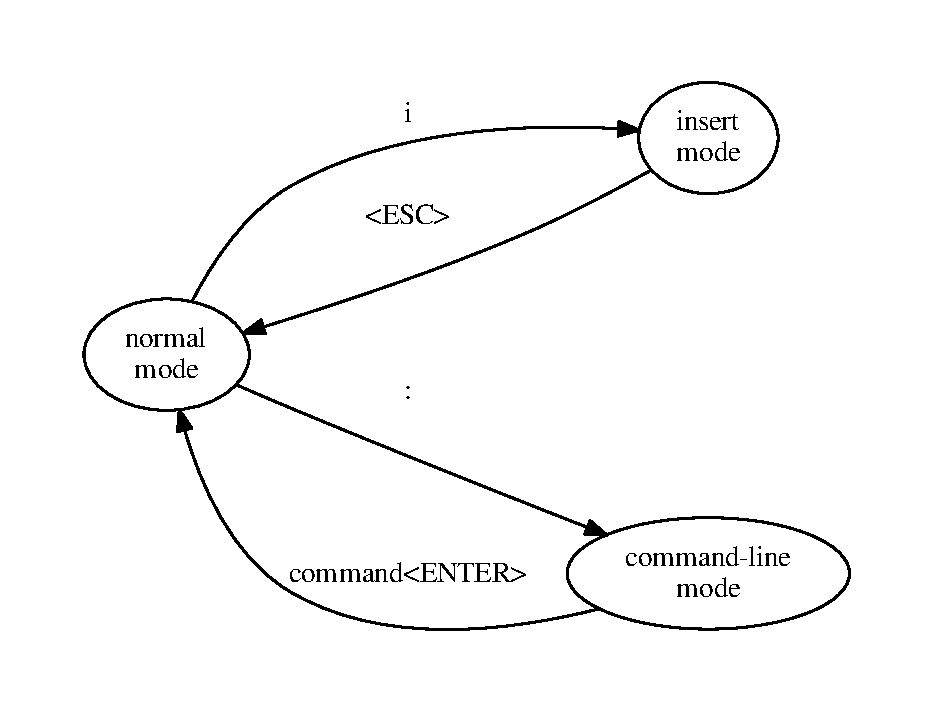
\includegraphics[width=.9\linewidth]{img/vimode-basic.pdf}
\end{frame}
\subsection{vim移动}
\label{sec-4-2}
\begin{frame}[fragile]
\frametitle{移动光标(normal模式)}
\label{sec-4-2-1}
\begin{columns}
\begin{column}{0.5\textwidth}
%% 移动光标
\label{sec-4-2-1-1}


\begin{verbatim}
j      #光标下移一行
k      #光标上移一行
h      #光标左移一个字符
l      #光标右移一个字符
5k     #光标下移5行
10h    #光标左移10个字符
^      #行首(文本)
0      #行首
$      #行尾
\end{verbatim}
\end{column}
\begin{column}{0.5\textwidth}
%% 图示
\label{sec-4-2-1-2}

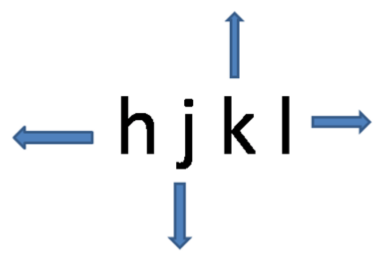
\includegraphics[width=.9\linewidth]{img/vi-move.png}
\end{column}
\end{columns}
\end{frame}
\begin{frame}[fragile]
\frametitle{移动光标}
\label{sec-4-2-2}
%% 移动光标
\label{sec-4-2-2-1}


\begin{verbatim}
Ctrl-b     #上一页(backward)
Ctrl-f     #下一页(forward)
15G        #光标移至第15行
gg         #首行
G          #尾行
H          #屏幕首行(high)
M          #屏幕中间(middle)
L          #屏幕底行(low)
Ctrl-o     #回到上一位置
Ctrl-i     #回到下一位置
Ctrl-g     #查看当前光标位置
\end{verbatim}
\note{示例文件

file: learn-vim
content:
today, we will start to learn using vim editor.

when you firest start into vim, 
you will find that when you type some letters on your keyborad, 
the editor seems have no respones to your input, 

what happened? don't panic,
vim is a mode text editor which is very differnet from other text editors. 
when you start vim, you will into a special status which is named normal mode, 
in this mode, whatever you type are interpreted as a command instead of the content. 

then how can we begin to input our text? 
is is easy, just type letter i, which means the command insert, 
so you will be bring into the second status called insert mode, 
in this mode, you can input what you want to the file you are editing.

after adding some content to your file, you want to save your work, 
but you find that there is no save button avaible, you are in confusion again.

so it is time to tell you the final basic mode: the command-line mode.
first, you must press the <ESC> key on the left top of your keyboard.
the <ESC> key can bring you back to the normal mode from any mode immediately.
then you should type the letter : now.

you can see the : display on the bottom of the editor, 
which means you have got into the command-line mode.

in this mode, we can input some command and then press enter key to excute it.
for now, we want to save our file, 

so we can input w followed by a file name you want, for example, myfile.
then press the enter key, 
the content you just input in the insert mode will be saved to the file.
at the same time, you have gont back to the normal mode again.

you can repeat switching among these three modes,
modify your content and save your modifications again and again.

but if you have finished all your edit work, how to quit vim?
it is simple as well, 

you can return to the normal mode, 
and input : to go into the command-line mode,
then type wq to save and quit your work, 
or type q! to quit vim without saving your last modifications.
}
\end{frame}
\begin{frame}[fragile]
\frametitle{移动光标}
\label{sec-4-2-3}
%% 移动光标
\label{sec-4-2-3-1}


\begin{verbatim}
b          #往前至单词开头 b (beginning)
w          #下一个单词 w (word)
e          #往后至单词尾部 e (end)
(          #上一句
)          #下一句
3(         #下3句
{          #上一段
}          #下一段
%          #配对括号
\end{verbatim}
\end{frame}
\subsection{vim编辑}
\label{sec-4-3}
\begin{frame}[fragile]
\frametitle{编辑命令}
\label{sec-4-3-1}
%% 编辑命令
\label{sec-4-3-1-1}


\begin{verbatim}
i    #在光标前插入
I    #在行首插入
a    #在光标后插入
A    #在行尾插入
o    #在光标下方插入新行
O    #在光标上方插入新行
r    #替换光标所在字符(单字符替换,且保持在normal模式)
R    #从光标所在位置开始向后替换
s    #删除光标所在字符并进入插入模式(可用多字符替换单字符)
S    #删除当前行并进入插入模式(替换整行)
x    #删除光标所在字符(向后删除,且保持在normal模式)
X    #删除光标前一字符(向前删除,且保持在normal模式)
\end{verbatim}
\end{frame}
\begin{frame}[fragile]
\frametitle{撤销与重做}
\label{sec-4-3-2}
\begin{exampleblock}{撤销}
\label{sec-4-3-2-1}


\begin{verbatim}
u            #撤销一次操作
U            #撤销对当前行的所有修改
:earlier 1f  #回到上次存盘时的状态
\end{verbatim}
\end{exampleblock}
\begin{block}{重做(要先有撤销操作才有效)}
\label{sec-4-3-2-2}


\begin{verbatim}
Ctrl+r       #重做最近被撤销一次操作
:redo  5     #重做最近撤销的5步操作
:later 1f    #进到下次存盘时的状态
\end{verbatim}
\end{block}
\end{frame}
\begin{frame}[fragile]
\frametitle{撤销分支}
\label{sec-4-3-3}
\begin{columns}
\begin{column}{0.3\textwidth}
%% 示例
\label{sec-4-3-3-1}

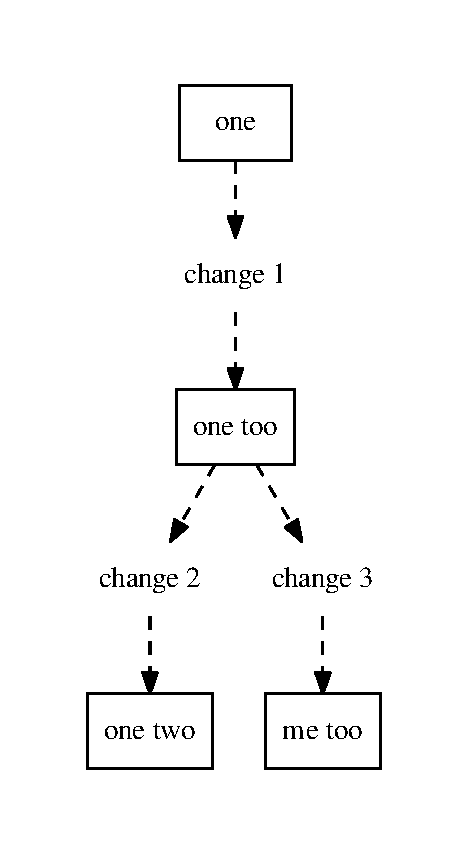
\includegraphics[width=.9\linewidth]{img/undotree.pdf}
\end{column}
\begin{column}{0.7\textwidth}
\begin{itemize}

\item 示例\\
\label{sec-4-3-3-2}%
\begin{verbatim}
1. 在me too按u,回到one too
2. 再次按u,回到one
3. 按Ctrl-r,进到one two
4. 再按Ctrl-r,进到me two
u和Ctrl-r只能在当前分支内上下移动
g-          #沿时间轴回退1步
g+          #沿时间轴前进1步
:undolist   #查看undo分支树页节点列表
:undo 2     #回到分支2(one two)
:earlier 5m #回退至5分钟前的状态
:later 10s  #前进至10秒后的状态
\end{verbatim}
\end{itemize} % ends low level
\end{column}
\end{columns}
\end{frame}
\subsection{vim语言}
\label{sec-4-4}
\begin{frame}[fragile]
\frametitle{动词}
\label{sec-4-4-1}
\begin{columns}
\begin{column}{0.6\textwidth}
\begin{exampleblock}{动词代表操作}
\label{sec-4-4-1-1}


\begin{verbatim}
c   #修改(change)
d   #删除(delete)
r   #替换(replace)
y   #复制(yank)
v   #选取(visual select)
p   #(paste),在光标右/下方粘贴
P   #(Paste),在光标左/上方粘贴
>   #缩进
<   #反缩进
\end{verbatim}
\end{exampleblock}
\end{column}
\begin{column}{0.4\textwidth}
\begin{block}{行操作}
\label{sec-4-4-1-2}


\begin{verbatim}
cc  #修改当前行
dd  #删除当前行
yy  #复制当前行
3dd #删除3行
5yy #复制5行
4>> #缩进4行
<<  #反缩进当前行
\end{verbatim}
\end{block}
\end{column}
\end{columns}
\end{frame}
\begin{frame}[fragile]
\frametitle{名词和介词}
\label{sec-4-4-2}
\begin{columns}
\begin{column}{0.5\textwidth}
\begin{exampleblock}{名词代表文本对象}
\label{sec-4-4-2-1}


\begin{verbatim}
w   #一个单词(word)
s   #一个句子(sentence)
p   #一个段落(paragraph)
t   #一个标签(tag)
"   #一个"..."文本块
{   #一个{...}文本块
\end{verbatim}
\end{exampleblock}
\end{column}
\begin{column}{0.5\textwidth}
\begin{block}{介词界定了范围或位置}
\label{sec-4-4-2-2}


\begin{verbatim}
i   #在...内(inside)
a   #环绕...(around)
t   #到...前(to)
f   #到...上(forward)
\end{verbatim}
\end{block}
\end{column}
\end{columns}
\end{frame}
\begin{frame}
\frametitle{名词和介词}
\label{sec-4-4-3}

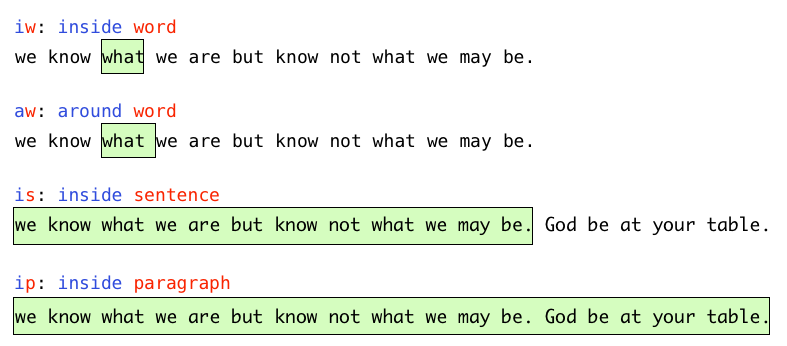
\includegraphics[width=.9\linewidth]{img/vimlang1.png}
\end{frame}
\begin{frame}[fragile]
\frametitle{组词为句}
\label{sec-4-4-4}
\begin{exampleblock}{动词+介词+名词}
\label{sec-4-4-4-1}


\begin{verbatim}
dip #删除一个段落:delete inside paragraph
vis #选取一个句子:visual select inside sentence
ciw #修改一个单词:change inside word
caw #修改一个单词:change around word
dtx #删除文本直到字符x(不包括x):delete to x
dfx #删除文本直到字符x(包括x):delete forward x
>ap #缩进一个段落
>i{ #缩进一个{}块内的内容
\end{verbatim}
\end{exampleblock}
\end{frame}
\begin{frame}[fragile]
\frametitle{数词:数词可修饰名词或动词}
\label{sec-4-4-5}
\begin{exampleblock}{数词修饰名词:动词+数词+名词}
\label{sec-4-4-5-1}


\begin{verbatim}
c3w #修改3个单词:change three words
d2w #删除2个单词:delete two words
\end{verbatim}
\end{exampleblock}
\begin{block}{数词修饰动词:数词+动词+名词}
\label{sec-4-4-5-2}


\begin{verbatim}
2dw #两次删除单词:twice delete word
3x  #三次删除字符:three times delete character
\end{verbatim}
\end{block}
\end{frame}
\begin{frame}[fragile]
\frametitle{更多例子}
\label{sec-4-4-6}
\begin{columns}
\begin{column}{0.5\textwidth}
\begin{exampleblock}{动词+位置}
\label{sec-4-4-6-1}


\begin{verbatim}
dl   #向右删除字符,即x
dh   #向左删除字符,即X
yj   #复制当前行,即yy
yk   #复制上一行
dfi  #向右删除至字母i
2yj  #同上
y2j  #同上
dG   #向下删除至结尾
c4G  #修改至第4行
d$   #删除至行尾
c^   #修改至行首
\end{verbatim}
\end{exampleblock}
\end{column}
\begin{column}{0.5\textwidth}
\begin{block}{动词+名词}
\label{sec-4-4-6-2}


\begin{verbatim}
2cw  #向右修改两个单词
d2b  #向左删除两个单词
c)   #修改至句尾
y{   #复制至段首
yaw  #复制当前单词
2daw #删除两个单词
yas  #复制当前句子
yap  #复制光标所在段落
2yap #复制两个段落
da<  #删除<...>
ci"  #修改"..."内的...
\end{verbatim}
\end{block}
\end{column}
\end{columns}
\end{frame}
\begin{frame}[fragile]
\frametitle{可视模式}
\label{sec-4-4-7}
\begin{itemize}

\item 进入可视模式后可通过移动光标可用于选择大块文本
\label{sec-4-4-7-1}%
\begin{exampleblock}{进入可视模式}
\label{sec-4-4-7-1-1}


\begin{verbatim}
v          #字符可视模式
Shift-v    #行可视模式
Ctrl-v     #块可视模式
\end{verbatim}
\end{exampleblock}

\item 对文本块的操作步骤:
\label{sec-4-4-7-2}%
\begin{enumerate}
\item 将光标移动至文本块的开始位置
\item 进入可视模式
\item 移动光标选择文本块
\item 按c修改,按y复制,按d剪切,按<ESC>返回normal模式
\end{enumerate}
\end{itemize} % ends low level
\end{frame}
\begin{frame}[fragile]
\frametitle{其他编辑操作}
\label{sec-4-4-8}
\begin{itemize}

\item 转换大小写\\
\label{sec-4-4-8-1}%
\begin{verbatim}
~
\end{verbatim}

\item 将下一行与当前行合并\\
\label{sec-4-4-8-2}%
\begin{verbatim}
J
\end{verbatim}

\item 使用缩写\\
\label{sec-4-4-8-3}%
\begin{verbatim}
:ab nos network operating system
输入nos并按空格键
:iab cn computer networks
输入cn并按空格键
注意:iab缩写仅在insert模式中有效
\end{verbatim}
\end{itemize} % ends low level
\end{frame}
\subsection{vim搜索与替换}
\label{sec-4-5}
\begin{frame}[fragile]
\frametitle{搜索}
\label{sec-4-5-1}
\begin{itemize}

\item 前向搜索\\
\label{sec-4-5-1-1}%
\begin{verbatim}
/mode   #从当前位置向下搜索字符串mode
?mode  #从当前位置向上搜索字符串mode
n       #下一个
N       #上一个
\end{verbatim}

\item 搜索光标所在单词\\
\label{sec-4-5-1-2}%
\begin{verbatim}
*      #下一个
#      #上一个
\end{verbatim}

\item 在当前行内搜索光标所在字符\\
\label{sec-4-5-1-3}%
\begin{verbatim}
fd      #下一个d
Fd      #上一个d
;       #重复f/F命令
,       #反向重复f/F命令
\end{verbatim}
\end{itemize} % ends low level
\end{frame}
\begin{frame}[fragile]
\frametitle{搜索替换}
\label{sec-4-5-2}
%% 示例
\label{sec-4-5-2-1}


\begin{verbatim}
:s/old/new        #将当前行第一次出现的old替换为new
:s/old/new/g      #将当前行所有的old替换为new
:3,10s/old/new/g  #将3到50行内所有old替换为new
:%s/old/new/g     #将当前文档所有的old替换为new
:%s/old/new/gc    #同上,但每次替换需要用户确认
\end{verbatim}
\end{frame}
\subsection{vim进阶}
\label{sec-4-6}
\begin{frame}[fragile]
\frametitle{重复上次编辑操作}
\label{sec-4-6-1}
\begin{itemize}

\item .命令
\label{sec-4-6-1-1}%
\begin{itemize}

\item 从进入insert模式的命令开始到按<ESC>键回到normal模式中为止,所有的动作(其中没有发生过光标移动动作)被当作一次操作,可以用.重复执行
\label{sec-4-6-1-1-1}%

\item 如果进入insert模式后做了多次光标移动动作,则每两次光标移动之间的动作被当作一次操作,因此按<ESC>键回到normal模式后,用.只能重复insert模式中最后一次光标移动之后的所有动作
\label{sec-4-6-1-1-2}%

\item 例:在文件的每行开始增加”todo: “\\
\label{sec-4-6-1-1-3}%
\begin{verbatim}
gg     #光标移至首行
Itodo: #在行首添加todo:
<ESC>  #回到normal模式
j.     #下一行重复上一步操作
j.     #同上
\end{verbatim}
\end{itemize} % ends low level
\end{itemize} % ends low level
\end{frame}
\begin{frame}[fragile]
\frametitle{书签}
\label{sec-4-6-2}
\begin{itemize}

\item 有时需要临时离开当前编辑位置,转到文档的其他位置进行编辑,编辑完成后,如何快速地从其他位置回到原来的位置呢?
\label{sec-4-6-2-1}%
\end{itemize} % ends low level
\begin{exampleblock}{设置书签}
\label{sec-4-6-2-2}


\begin{verbatim}
ma    #标记(mark)当前位置,标记名可为a-zA-Z
G     #将光标移至末行
'a    #快速回到标记a所在行行首
`a    #快速回到标记a的准确位置
\end{verbatim}
\end{exampleblock}
\end{frame}
\begin{frame}[fragile]
\frametitle{寄存器}
\label{sec-4-6-3}
\begin{itemize}

\item 复制或删除的内容可以分别放在多个寄存器中,将来可进行选择性粘贴
\label{sec-4-6-3-1}%
\end{itemize} % ends low level
\begin{exampleblock}{示例:使用寄存器实现选择性粘贴}
\label{sec-4-6-3-2}


\begin{verbatim}
"a4yy  #复制4行至寄存器a
"b2dd  #删除2行至寄存器b
"cyap  #复制1段至寄存器c
"ap    #粘帖寄存器a中的内容
"bp    #粘帖寄存器b中的内容
"cp    #粘贴寄存器c中的段落
\end{verbatim}
\end{exampleblock}
\end{frame}
\begin{frame}[fragile]
\frametitle{录制与重放宏操作}
\label{sec-4-6-4}
\begin{itemize}

\item vim可以把多步操作录制为单个宏,并可以播放宏以重复该多步操作
\label{sec-4-6-4-1}%
\end{itemize} % ends low level
\begin{exampleblock}{示例:为单词添加一对双引号}
\label{sec-4-6-4-2}


\begin{verbatim}
qa       #开始录制宏a
b        #移至单词开头
i"<ESC>  #插入一个双引号
e        #移至单词结尾
a"<ESC>  #追加一个双引号
q        #结束录制
         #将光标移至另一个单词
@a       #播放宏a
\end{verbatim}
\end{exampleblock}
\end{frame}
\begin{frame}[fragile]
\frametitle{执行shell命令}
\label{sec-4-6-5}
\begin{exampleblock}{在vim中执行shell命令}
\label{sec-4-6-5-1}


\begin{verbatim}
:!cal      #执行cal命令
:sh        #暂时切换到shell,按Ctrl-d返回
!!uname -r #执行命令并用其输出替换当前行
\end{verbatim}
\end{exampleblock}
\end{frame}
\begin{frame}[fragile]
\frametitle{文件处理}
\label{sec-4-6-6}
\begin{exampleblock}{文件处理}
\label{sec-4-6-6-1}


\begin{verbatim}
:cd dir1       #切换到目录dir1
:pwd           #查看当前目录
:r file1        #在当前行后插入文件file1
:10 r file2     #在第10行后插入文件file2
:w file3        #将当前文件(另)存为file3
:4,20 w file4   #将4至20行另存为file4
\end{verbatim}
\end{exampleblock}
\end{frame}
\begin{frame}[fragile]
\frametitle{文件加密}
\label{sec-4-6-7}
\begin{exampleblock}{加密}
\label{sec-4-6-7-1}


\begin{verbatim}
:X (大写)
:set key=123
\end{verbatim}
\end{exampleblock}
\begin{block}{解除加密}
\label{sec-4-6-7-2}


\begin{verbatim}
:set key=     #设置key值为空
\end{verbatim}
\end{block}
\end{frame}
\begin{frame}[fragile]
\frametitle{vim与多文件处理}
\label{sec-4-6-8}
\begin{exampleblock}{多文件}
\label{sec-4-6-8-1}


\begin{verbatim}
vim file1 file2 file3
:ls       #列出所有打开的文件
:b3       #跳至第3个文件
:n        #切换至下一文件
:N        #切换至上一文件
:e file2  #切换至指定文件
\end{verbatim}
\end{exampleblock}
\end{frame}
\begin{frame}[fragile]
\frametitle{vim与多窗口处理}
\label{sec-4-6-9}
\begin{columns}
\begin{column}{0.5\textwidth}
\begin{exampleblock}{窗口操作}
\label{sec-4-6-9-1}


\begin{verbatim}
:new           #上下拆分
:vnew          #左右拆分
:sp/Ctrl-w s   #上下拆分
:vsp/Ctrl-w v  #左右拆分
:close/:q      #关闭当前窗口
Ctrl-w j/k/h/l #上下左右跳转
Ctrl-w         #跳至下一窗口
Ctrl-w Ctrl-w  #循环跳转
\end{verbatim}
\end{exampleblock}
\end{column}
\begin{column}{0.5\textwidth}
\begin{block}{窗口操作}
\label{sec-4-6-9-2}


\begin{verbatim}
Ctrl-w o      #仅显示当前窗口
Ctrl-w =      #所有窗口等大
Ctrl-w _      #当前窗口最大化
Ctrl-w +      #增大窗口
Ctrl-w -      #减小窗口
:resize 3     #调整窗口行数
Ctrl-w r      #旋转窗口顺序
Ctrl-w K      #当前窗口置顶
\end{verbatim}
\end{block}
\end{column}
\end{columns}
\end{frame}
\begin{frame}[fragile]
\frametitle{vim与多标签处理}
\label{sec-4-6-10}
\begin{exampleblock}{多标签}
\label{sec-4-6-10-1}


\begin{verbatim}
:tabnew           #创建新标签
:tabe[dit] file   #新标签编辑文件
:tabc[lose]/:q    #关闭标签
gt                #下一个标签
gT                #上一个标签
:tabm[ove] n      #当前标签移至位置n(从0开始)
\end{verbatim}
\end{exampleblock}
\end{frame}
\begin{frame}[fragile]
\frametitle{获取帮助}
\label{sec-4-6-11}
\begin{exampleblock}{获取帮助}
\label{sec-4-6-11-1}


\begin{verbatim}
vimtutor
:h
\end{verbatim}
\end{exampleblock}
\end{frame}
\begin{frame}[fragile]
\frametitle{vim配置}
\label{sec-4-6-12}
\begin{itemize}

\item 临时配置
\label{sec-4-6-12-1}%
\end{itemize} % ends low level
\begin{exampleblock}{:set命令}
\label{sec-4-6-12-2}


\begin{verbatim}
:set nu[mber]   #显示行号
:set nonu[mber] #取消显示行号
:set ai         #自动缩进(auto indent)
:set noai       #取消自动缩进
:set cindent shiftwidth=4 #设置C语言风格
:set all        #查看所有可用选项
\end{verbatim}
\end{exampleblock}
\begin{itemize}

\item 永久配置
\label{sec-4-6-12-3}%
\begin{itemize}

\item 全局配置:/etc/vim/vimrc
\label{sec-4-6-12-3-1}%

\item 用户配置:\~{}/.vimrc
\label{sec-4-6-12-3-2}%
\end{itemize} % ends low level
\end{itemize} % ends low level
\end{frame}
\begin{frame}[fragile]
\frametitle{.vimrc配置文件示例}
\label{sec-4-6-13}
\begin{exampleblock}{C编程配置}
\label{sec-4-6-13-1}


\begin{verbatim}
syntax on
set cindent
set nu
set tabstop=4
set shiftwidth=4
colo evening

map <F5> :call Run()<CR>
func! Run()
  exec "w"
  exec "!g++ -Wall % -o %<"
  exec "!./%<"
endfunc
\end{verbatim}
\end{exampleblock}
\end{frame}
\begin{frame}
\frametitle{vim键盘图}
\label{sec-4-6-14}

\begin{center}
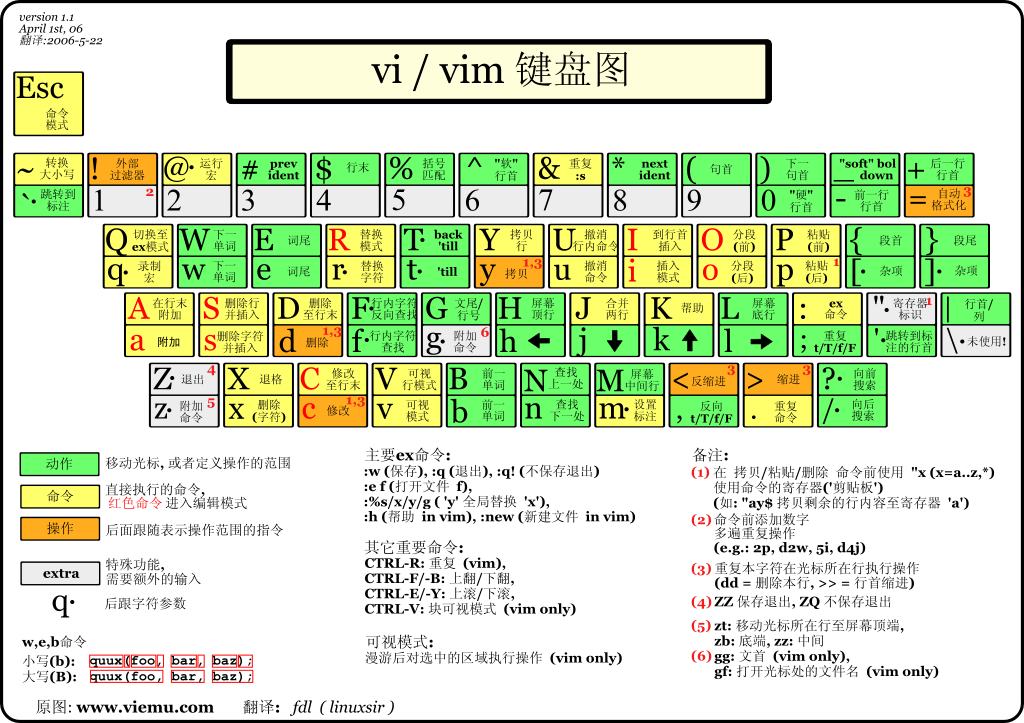
\includegraphics[width=.9\linewidth]{img/vim-keys.png}
\end{center}
\end{frame}

\end{document}
